%Slide template developed by Mark E. Fuller from examples and miscellany produced at RWTH Aachen
%(probably mostly from the work of Philippe Dreuw and Thomas Deselaers)
%This template copyright Mark E. Fuller, 2021 (mark.e.fuller@gmx.de)

\documentclass[10pt,presentation]{beamer}

\usepackage[utf8]{inputenc}

%%%%%%%%%%%%%%%%%%%%%%%%%%%%%%%%%%%%%
%% Select language
%%
%\usepackage[ngerman]{babel}        % Deutsch, neue Rechtschreibung
%\usepackage[hebrew,english]{babel}  %example of declaring multilingual document; last listed is ``dominant''
\usepackage[english]{babel}

%regional add-ons
    % Shekel symbol
\DeclareRobustCommand{\ILS}{
\includegraphics[height=\fontcharht\font`T]{figures/ILS_bold}}

\usetheme{technion}
\usepackage[T1]{fontenc}           % Font encoding (don't change!)
\usepackage{lmodern}               % Select Linux Modern Fonts (don't change)
\usepackage{sansmathfonts}         % Sans fonts in math environments
\usepackage{textcomp}              % fix 'missing font symbols' warning
\renewcommand{\rmdefault}{phv}     % Arial like (Helvetica)
\renewcommand{\sfdefault}{phv}     % Arial like (Helvetica)

%% graphics related packages
\usepackage{graphicx}              % needed to include graphics (don't change)
\usepackage{epstopdf}              % required to include eps files
%\usepackage{svg}                   % include svg files (requires Inkscape)
\usepackage{subfigure}             % option to layout figures in tabular environment
\usepackage[encoding,filenameencoding=utf8]{grffile} % allow utf8 file names in graphics´
\setbeamertemplate{caption}{\insertcaption} %no ``figure'' in caption
\usepackage{tikz}
\usepackage{curves}
\usepackage{pgfplots}

%%%%%%%%%%%%%%%%%%%%%%%%%%%%%%%%%%%%%
%% import packages for content
%%
\usepackage{listings}              % display code: for lstlisting and \lstinline|..|

% mathematics
\usepackage{amsmath}
\usepackage{amssymb}
\usepackage{sansmath}

% tabularx -> better tabular environment
\usepackage{tabularx}
    % tabularx modifications
\newcolumntype{L}{>{\raggedright\let\newline\\\arraybackslash\hspace{0pt}}X}
\newcolumntype{R}{>{\raggedleft\let\newline\\\arraybackslash\hspace{0pt}}X}
\newcolumntype{C}{>{\centering\let\newline\\\arraybackslash\hspace{0pt}}X}
    % center text vertically in tabularx(column)
%\renewcommand{\tabularxcolumn}[1]{>{\large}m{#1}}

% Nicer tables
\usepackage{booktabs}
    % adjust table rows -> call on frame with table
\newcommand{\fixbooktabsrowhight}{%
    \setlength{\aboverulesep}{0pt}
    \setlength{\belowrulesep}{0pt}
    \setlength{\extrarowheight}{.5ex}
}
\usepackage{multirow} % cells with multiple rows
\usepackage{scrextend} %needed for footnotes in tables

% Source, e.g. for images
\setbeamercolor{framesource}{fg=gray}
\setbeamerfont{framesource}{size=\tiny}

\usepackage[absolute,overlay]{textpos}
\newcommand{\source}[1]{\begin{textblock*}{\linewidth}(1ex,\paperheight-2.75em)
        \begin{beamercolorbox}[left]{framesource}
            \usebeamerfont{framesource}\usebeamercolor[fg]{framesource} Source: {#1}
        \end{beamercolorbox}
\end{textblock*}}

\usepackage{etoolbox}
%% short titles for toc \(sub)section[SHORTTITLE for toc]{LONGTITLE for slide}
\makeatletter
% Insert [short title] for \section in ToC
\patchcmd{\beamer@section}{{#2}{\the\c@page}}{{#1}{\the\c@page}}{}{}
% Insert [short title] for \section in Navigation
\patchcmd{\beamer@section}{{\the\c@section}{\secname}}{{\the\c@section}{#1}}{}{}
% Insert [short title] for \subsection in ToC
\patchcmd{\beamer@subsection}{{#2}{\the\c@page}}{{#1}{\the\c@page}}{}{}
% Insert [short title] for \subsection  in Navigation
\patchcmd{\beamer@subsection}{{\the\c@subsection}{#2}}{{\the\c@subsection}{#1}}{}{}
\makeatother

%easily format to multiple columns
\usepackage{multicol}

%properly display chemical formulas and structures
    % Formula subscripts using \ce{}
\usepackage[version=3]{mhchem} 
    % structure drawing package
%\usepackage{chemfig}
%\setchemfig{chemfig style={line width=1.0pt}, atom sep=2em, angle increment=30, bond join=true, arrow style={line width=1.0pt}, lewis sep=0.3em}
%\pgfplotsset{compat=1.13}
    % define repeated abbreviations
\newcommand{\nox}{NO$_x$}


% Bibliography and citations

%get proper bib with numbered entries
%\setbeamertemplate{bibliography item}{\insertbiblabel}

%footnote citations - replace \cite with \footcite or \footfullcite
\usepackage[backend=biber, style=chem-acs]{biblatex} %, style=authoryear-comp
\addbibresource{sample.bib}

%shrink citations
\setbeamerfont{footnote}{size=\tiny}

%bibliography/citation style
\setbeamertemplate{bibliography item}{\insertbiblabel}
\setbeamercolor{bibliography item}{fg=black}
\setbeamercolor*{bibliography entry author}{fg=black}


%some additional formatting
\newcommand{\red}[1]{\textcolor{red}{#1}} %easy red text
\usepackage{ulem}
\newcommand{\soutthick}[1]{%
	\renewcommand{\ULthickness}{1.6pt}%
	\sout{#1}%
	\renewcommand{\ULthickness}{.4pt}% Resetting to ulem default
}


%document header
\title{Progress in \soutthick{ Nitrogen } Novel Combustion Chemistry}
%\subtitle{Subtitle}
%\titlegraphic{}
\author{Mark E. Fuller, Ph.D.}
\email{fuller@technion.ac.il} % optionally
\institute{Dana Research Group: Fundamental and Applied Chemical Kinetics}
%\webaddress{www.informatik.rwth-aachen.de/mentoring} % overrides www.rwth-aachen.de
\date{\today}
\subject{Dana Technion presentation template}
\keywords{Technion, Latex Beamer, template}

%\logo{\vskip-2mm
\includegraphics[width=45mm]{../common/figures/Logos/RWTH/PCFC.png}\hspace{-2mm}} % optionally


%%%%%%%%%%%%%%%%%%%%%%%%%%%%%%%%%%%%%
%% configure template behaviour
%%-------------------------------
%%   secstart -- style of section start
%%               selectable parameters:
%%                 sectitle:  only provides section title
%%                 sectoc:    display section table of contents
%%                 <empty>:   display nothing on section start
\secstart{sectitle}
% disable PDF navigation icons
\setbeamertemplate{navigation symbols}{}

\begin{document}

\begin{frame}{Citations}
    \begin{itemize}
        \item Regular (end) citation\cite{Fuller.2014}
        \item Footnote\footfullcite{Fuller.2019}
    \end{itemize}
\end{frame}

\begin{frame}{Reaction Classes and Examples}
    \begin{multicols}{2}
    \begin{itemize}
        \item Hydrogen abstractions
        \begin{itemize}
            \item \ce{RH} + \ce{NO2} $\rightleftharpoons$ \ce{R} + \ce{HONO}
            \item \ce{RH} + \ce{NO2} $\rightleftharpoons$ \ce{R} + \ce{HNO2}
            \item \ce{RH} + \ce{NO} $\rightleftharpoons$ \ce{R} + \ce{HNO}
        \end{itemize}
        \item Nitrite/Nitrate/Nitro-/Nitroso- Compounds
        \begin{itemize}
            \item \ce{RONO} $\rightleftharpoons$ \ce{RO} + \ce{NO}
            \item \ce{RONO2} $\rightleftharpoons$ \ce{RO} + \ce{NO2}
            \item \ce{RNO2} $\rightleftharpoons$ \ce{R} + \ce{NO2}
            \item \ce{RNO} $\rightleftharpoons$ \ce{R} + \ce{NO}
        \end{itemize}
        \item Isomerizations  
        \begin{itemize}
            \item \ce{RONO} $\rightleftharpoons$ \ce{RNO2}
        \end{itemize}
        \item \ce{HONO} elimination
        \begin{itemize}
            \item \ce{RONO} $\rightleftharpoons$ alkene + \ce{HONO}
        \end{itemize}
        \item \nox\ cycling
        \begin{itemize}
            \item \ce{RO2} + \ce{NO} $\rightleftharpoons$ \ce{RO} + \ce{NO2}
            \item \ce{R} + \ce{NO2} $\rightleftharpoons$ \ce{RO} + \ce{NO}
        \end{itemize}
    \end{itemize}
    
    \columnbreak
    
    \null \vfill
    \begin{figure}
        \centering
        \resizebox{\columnwidth}{!}{
            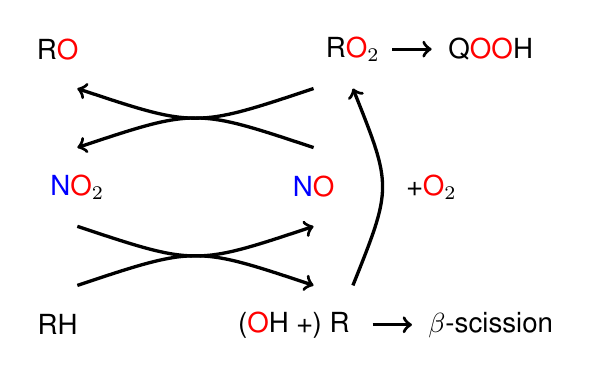
\begin{tikzpicture}
                %nox loop bounds
                \draw[->,very thick] (1,1) .. controls (2.5,0.5) .. (4,1);
                \draw[<-,very thick] (1,2) .. controls (2.5,2.5) .. (4,2);
                \draw (1,1.5) node {{\color{blue}N}{\color{red}O}$_2$};
                \draw (4,1.5) node {{\color{blue}N}{\color{red}O}};
                
                \draw[->,very thick] (1,0.25) .. controls (2.5,0.75) .. (4,0.25);
                \draw (0.75,-0.25) node {\ce{RH}};
                \draw (3.75,-0.25) node {({\color{red}O}H +) \ce{R} };
                
                \draw[<-,very thick] (1,2.75) .. controls (2.5,2.25) .. (4,2.75);
                \draw (0.75,3.25) node {R{\color{red}O}};
                \draw (4.5,3.25) node {R{\color{red}O}$_2$}; 
                
                \draw[->,very thick] (4.5,0.25) .. controls (5,1.5) .. (4.5,2.75); 
                \draw (5.5,1.5) node {+{\color{red}O}$_2$};
                
                \draw[->,very thick] (5,3.25)--(5.5,3.25); 
                \draw (6.25,3.25) node {Q{\color{red}O}{\color{red}O}H};
                
                \draw[->,very thick] (4.75,-0.25)--(5.25,-0.25); 
                \draw (6.25,-0.25) node {$\beta$-scission};
            \end{tikzpicture}
        }
        \caption{And when \ce{RH} is replaced with \ce{QOOH} or \ce{OOQOOH}?}
        \label{fig:NOx_cycle}
    \end{figure}
    \vfill \null
    
    \end{multicols}
\end{frame}

\begin{frame}{Progress on \nox-Cycling}
	\begin{figure}
		\centering
        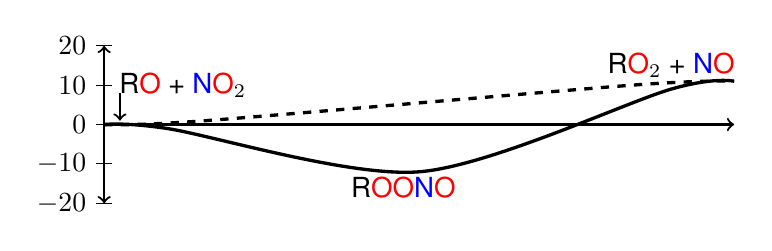
\begin{tikzpicture}[yscale = 0.5]
            %draw coordinate axis with labels
            %as above, not so many label, so they are manual here (e.g. make log)
            \draw[->,thick] (0,0) -- coordinate (x axis mid) (8,0);
            \draw[<->,thick] (0,2) -- coordinate (y axis mid)(0,-2);
            %\draw[gray, dashed](0,\ymax) grid (\Px,\ymin);
            \foreach \y/\ytext in {2/20, 1/10,0/0,-1/-10,-2/-20} \draw (3pt,\y cm) -- (-3pt,\y cm) node[anchor=east] {{$\ytext$}};
            
            %Text Labels
            %reactant side: placement will need to be adjusted for path lines
            \node [scale = 1.0,black] at (1.0, 1.0) {{R{\color{red}O} + {{\color{blue}N}{\color{red}O}$_2$}}};
            \node [scale = 1.0,black] at (7.2, 1.5){{R{\color{red}O}$_2$ + {{\color{blue}N}{\color{red}O}}}};      	
            \node [scale = 1.0,black] at (3.8, -1.60) {{R{\color{red}OO}{{\color{blue}N}{\color{red}O}}}};
            \draw[->,thick] (0.2,0.8) --(0.2,0.1);

            %links
            \draw[black, very thick] plot [smooth] coordinates {(0.0,0.0)(0.8,-0.1)(4.0, -1.2)(7.2,0.9)(8.0, 1.1)};
            \draw[black, very thick, dashed] plot [smooth] coordinates {(0.0,0.0)(1.3,0.1)(6.7,1.0)(8.0, 1.1)};
        \end{tikzpicture}
		\caption{Generalized potential energy surface for alkoxy radical (RO) + \ce{NO2} system. Energies in kcal/mol.
			Well-skipping occurs at virtually all combustion-relevant temperatures and pressures.}
		\label{fig:NOx-Cycle_PES}
	\end{figure}
\begin{tabular}{crrr}
	\toprule
	Reaction & \multicolumn{1}{c}{$A$} & \multicolumn{1}{c}{$n$} & \multicolumn{1}{c}{$E_a$}\\
	\midrule
	\ce{CH3O2} + \ce{NO} $\rightleftharpoons$ \ce{CH3O} + \ce{NO2} & 4.62E+15 & -0.38 & 97.8\\
	\ce{C2H5O2} + \ce{NO} $\rightleftharpoons$ \ce{C2H5O} + \ce{NO2} & 2.11E+14 & -0.12 & -470.6\\
	\ce{NC3H7O2} + \ce{NO} $\rightleftharpoons$ \ce{NC3H7O} + \ce{NO2} & 1.07E+14 & -0.25 & -1302.0\\
	\bottomrule
\end{tabular}	

Units: centimeters, kelvin, calories, moles
\end{frame}


\printbibliography

\end{document}
